\documentclass[a4paper]{article}

\usepackage[T1]{fontenc}
\usepackage[utf8]{inputenc}
\usepackage[italian]{babel}
\usepackage[a4paper]{geometry}
\usepackage[hidelinks]{hyperref}
\usepackage{eurosym}
\usepackage{caption, subcaption}
\usepackage{tikz, circuitikz}
\usepackage{pgf-umlcd, pgf-umlsd}

\renewcommand{\umltextcolor}{black}
\renewcommand{\umldrawcolor}{black}
\renewcommand{\umlfillcolor}{white}

\setlength{\parskip}{1.2ex}
\setlength{\parindent}{0em}
\clubpenalty = 100
\widowpenalty = 100

\title{CHIP-8 STM32}
\date{\today}
\author{Federico Bruzzone, Lorenzo Ferrante, Andrea Longoni \\
\footnotesize \texttt{\{federico.bruzzone, lorenzo.ferrante1, andrea.longoni3\}@studenti.unimi.it} \\ }

\begin{document}
\maketitle

\section{Introduzione}

CHIP-8 è un linguaggio di programmazione creato a metà degli anni '70 da
Joseph Weisbecker per semplificare lo sviluppo di videogiochi per microcomputer
a 8 bit. I programmi CHIP-8 vengono interpretati da una macchina virtuale che è
stata estesa parecchie volte nel corso degli anni, tra le versioni più adottate
citiamo S-CHIP e la più recente XO-CHIP.

La semplicità dell'interprete in aggiunta alla sua lunga storia e popolarità
hanno fatto sì che emulatori e programmi CHIP-8 vengano realizzati ancora oggi.
Nel corso degli anni molti videogiochi storici sono stati "portati" su CHIP-8
tra cui Pong, Space Invaders e Tetris.

Lo scopo del progetto è quello di costruire un emulatore CHIP-8 e S-CHIP in
grado di funzionare su un microcontrollore STM32.

\section{Hardware}

% TODO

\begin{figure}
\begin{center}
    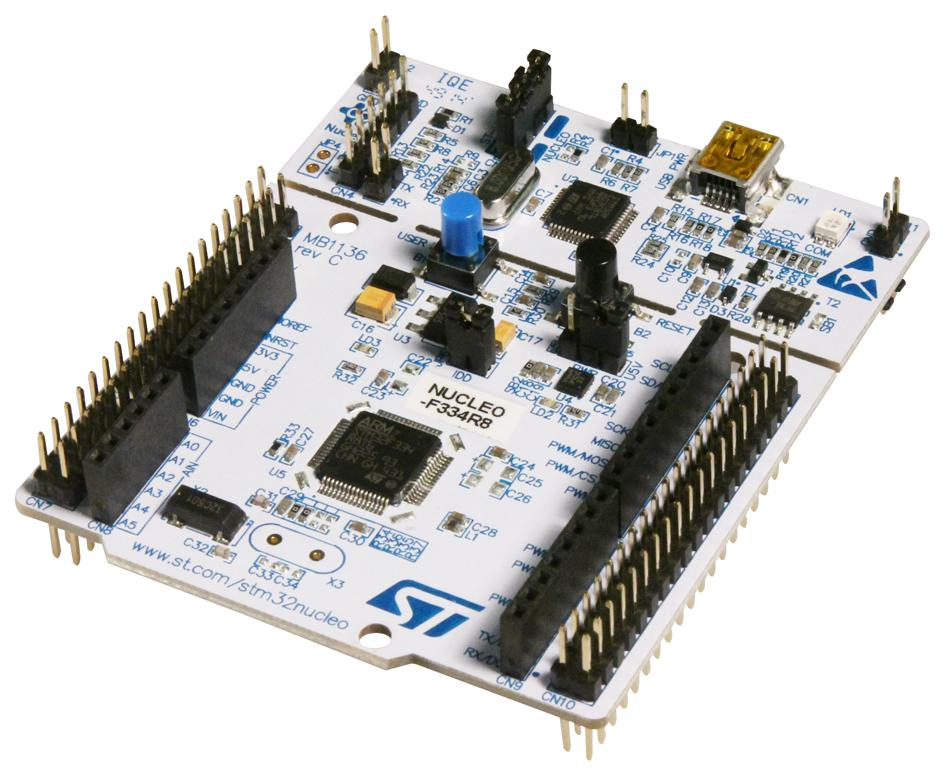
\includegraphics[scale=0.20]{figures/stm32f334.jpg}
\end{center}
\caption{Il microcontrollore \texttt{STM32F334R8T6}.}
\label{fig:weact_blackpill}
\end{figure}

\begin{figure}[h]
    \begin{subfigure}[b]{0.45\textwidth}
        \begin{center}
            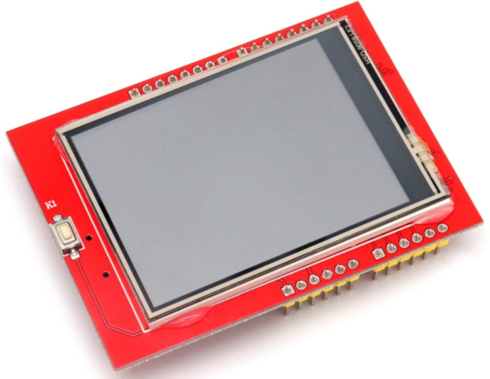
\includegraphics[scale=0.4]{figures/ili9341.png}
        \end{center}
        \caption{Lo schermo ILI9341.}
        \label{fig:ili9341}
    \end{subfigure}
    \hfill
    \begin{subfigure}[b]{0.45\textwidth}
        \begin{center}
            \begin{tikzpicture}[x=0.015cm, y=0.015cm, scale=0.75, transform shape]
                \draw   (120, 90) -- (320,90) -- (320,480) -- (120,480) -- cycle ;

\draw  [fill={rgb, 255:red, 255; green, 255; blue, 255 }  ,fill opacity=1 ]  (90,100)  --  (200,100) -- (200,130) --  (90,130) -- cycle;
\draw  [fill={rgb, 255:red, 255; green, 255; blue, 255 }  ,fill opacity=1 ]  (90,130)  --  (200,130) -- (200,160) --  (90,160) -- cycle;
\draw  [fill={rgb, 255:red, 255; green, 255; blue, 255 }  ,fill opacity=1 ]  (90,160)  --  (200,160) -- (200,190) --  (90,190) -- cycle;
\draw  [fill={rgb, 255:red, 255; green, 255; blue, 255 }  ,fill opacity=1 ]  (90,190)  --  (200,190) -- (200,220) --  (90,220) -- cycle;
\draw  [fill={rgb, 255:red, 255; green, 255; blue, 255 }  ,fill opacity=1 ]  (90,220)  --  (200,220) -- (200,250) --  (90,250) -- cycle;
\draw  [fill={rgb, 255:red, 255; green, 255; blue, 255 }  ,fill opacity=1 ]  (90,250)  --  (200,250) -- (200,280) --  (90,280) -- cycle;
\draw  [fill={rgb, 255:red, 255; green, 255; blue, 255 }  ,fill opacity=1 ]  (90,280)  --  (200,280) -- (200,310) --  (90,310) -- cycle;
\draw  [fill={rgb, 255:red, 255; green, 255; blue, 255 }  ,fill opacity=1 ]  (90,310)  --  (200,310) -- (200,340) --  (90,340) -- cycle;
\draw  [fill={rgb, 255:red, 255; green, 255; blue, 255 }  ,fill opacity=1 ]  (90,340)  --  (200,340) -- (200,370) --  (90,370) -- cycle;
\draw  [fill={rgb, 255:red, 255; green, 255; blue, 255 }  ,fill opacity=1 ]  (90,370)  --  (200,370) -- (200,400) --  (90,400) -- cycle;
\draw  [fill={rgb, 255:red, 255; green, 255; blue, 255 }  ,fill opacity=1 ]  (90,400)  --  (200,400) -- (200,430) --  (90,430) -- cycle;
\draw  [fill={rgb, 255:red, 255; green, 255; blue, 255 }  ,fill opacity=1 ]  (90,430)  --  (200,430) -- (200,460) --  (90,460) -- cycle;

\draw  [fill={rgb, 255:red, 255; green, 255; blue, 255 }  ,fill opacity=1 ] (250,100)  --  (380,100) -- (380,130) --  (250,130) -- cycle;
\draw  [fill={rgb, 255:red, 255; green, 255; blue, 255 }  ,fill opacity=1 ] (250,130)  --  (380,130) -- (380,160) --  (250,160) -- cycle;
\draw  [fill={rgb, 255:red, 255; green, 255; blue, 255 }  ,fill opacity=1 ] (250,160)  --  (380,160) -- (380,190) --  (250,190) -- cycle;
\draw  [fill={rgb, 255:red, 255; green, 255; blue, 255 }  ,fill opacity=1 ] (250,190)  --  (380,190) -- (380,220) --  (250,220) -- cycle;
\draw  [fill={rgb, 255:red, 255; green, 255; blue, 255 }  ,fill opacity=1 ] (250,220)  --  (380,220) -- (380,250) --  (250,250) -- cycle;
\draw  [fill={rgb, 255:red, 255; green, 255; blue, 255 }  ,fill opacity=1 ] (250,250)  --  (380,250) -- (380,280) --  (250,280) -- cycle;
\draw  [fill={rgb, 255:red, 255; green, 255; blue, 255 }  ,fill opacity=1 ] (250,280)  --  (380,280) -- (380,310) --  (250,310) -- cycle;
\draw  [fill={rgb, 255:red, 255; green, 255; blue, 255 }  ,fill opacity=1 ] (250,310)  --  (380,310) -- (380,340) --  (250,340) -- cycle;
\draw  [fill={rgb, 255:red, 255; green, 255; blue, 255 }  ,fill opacity=1 ] (250,340)  --  (380,340) -- (380,370) --  (250,370) -- cycle;


\draw (90,460) node [anchor=north west][inner sep=0.75pt]   [align=left] {$\displaystyle SD\_SCK$};
\draw (90,430) node [anchor=north west][inner sep=0.75pt]   [align=left] {$\displaystyle SD\_DO$};
\draw (90,400) node [anchor=north west][inner sep=0.75pt]   [align=left] {$\displaystyle SD\_DI$};
\draw (90,370) node [anchor=north west][inner sep=0.75pt]   [align=left] {$\displaystyle SD\_SS$};
\draw (90,340) node [anchor=north west][inner sep=0.75pt]   [align=left] {$\displaystyle LCD\_D1$};
\draw (90,310) node [anchor=north west][inner sep=0.75pt]   [align=left] {$\displaystyle LCD\_D0$};
\draw (90,280) node [anchor=north west][inner sep=0.75pt]   [align=left] {$\displaystyle LCD\_D7$};
\draw (90,250) node [anchor=north west][inner sep=0.75pt]   [align=left] {$\displaystyle LCD\_D6$};
\draw (90,220) node [anchor=north west][inner sep=0.75pt]   [align=left] {$\displaystyle LCD\_D4$};
\draw (90,190) node [anchor=north west][inner sep=0.75pt]   [align=left] {$\displaystyle LCD\_D5$};
\draw (90,160) node [anchor=north west][inner sep=0.75pt]   [align=left] {$\displaystyle LCD\_D3$};
\draw (90,130) node [anchor=north west][inner sep=0.75pt]   [align=left] {$\displaystyle LCD\_D2$};

\draw (250,370) node [anchor=north west][inner sep=0.75pt]   [align=left] {$\displaystyle 3.3V$};
\draw (250,340) node [anchor=north west][inner sep=0.75pt]   [align=left] {$\displaystyle 5V$};
\draw (250,310) node [anchor=north west][inner sep=0.75pt]   [align=left] {$\displaystyle GND$};
\draw (250,280) node [anchor=north west][inner sep=0.75pt]   [align=left] {$\displaystyle LCD\_RD$};
\draw (250,250) node [anchor=north west][inner sep=0.75pt]   [align=left] {$\displaystyle LCD\_WR$};
\draw (250,220) node [anchor=north west][inner sep=0.75pt]   [align=left] {$\displaystyle LCD\_RS$};
\draw (250,190) node [anchor=north west][inner sep=0.75pt]   [align=left] {$\displaystyle LCD\_CS$};
\draw (250,160) node [anchor=north west][inner sep=0.75pt]   [align=left] {$\displaystyle LCD\_RST$};
\draw (250,130) node [anchor=north west][inner sep=0.75pt]   [align=left] {$\displaystyle F\_CS$};

            \end{tikzpicture}
        \end{center}
        \caption{Pinout dello schermo \texttt{ILI9341}.}
        \label{fig:pinout_ili}
    \end{subfigure}
\end{figure}

\subsection{Materiali e costi} % ALT: Componenti e costi / Componenti utilizzati e relativi costi

\begin{center}
    \begin{table}[ht]
        \centering
        \begin{tabular}{|llll|l|}
            \hline
            \multicolumn{1}{|l|}{\textbf{Descrizione}}          & \multicolumn{1}{l|}{\textbf{Modello}}       & \multicolumn{1}{l|}{\textbf{Costo unitario}} & \textbf{Unità} & \textbf{Costo} \\ \hline
            \multicolumn{1}{|l|}{Microcontrollore}       & \multicolumn{1}{l|}{STM32 F334R8T6}         & \multicolumn{1}{l|}{14.99}                   & 1               & 14.99          \\ \hline
            \multicolumn{1}{|l|}{Schermo}                & \multicolumn{1}{l|}{ILI9341 2.4"}           & \multicolumn{1}{l|}{6.50}                    & 1               & 6.50           \\ \hline
            \multicolumn{1}{|l|}{Tastierino}          & \multicolumn{1}{l|}{Matrix keypad 4$\times$4} & \multicolumn{1}{l|}{3.99}                    & 1               & 3.99           \\ \hline
            \multicolumn{1}{|l|}{Beeper}                 & \multicolumn{1}{l|}{}                       & \multicolumn{1}{l|}{0.99}                    & 1               & 0.99           \\ \hline
            \multicolumn{1}{|l|}{Breadboard e cablaggio} & \multicolumn{1}{l|}{}                       & \multicolumn{1}{l|}{4.99}                    & 1               & 4.99           \\ \hline
            \multicolumn{4}{|r|}{\textbf{Totale}}                                                      & 31.50\euro    \\ \hline
        \end{tabular}
        \caption{
            Materiali utilizzati per la costruzione del progetto. I costi indicati provengono da negozi online come Amazon e eBay.
        }
    \end{table}
\end{center}

\section{Software}

% TODO

\subsection{Emulatore} % ALT: Emulatore CHIP-8 / Interprete CHIP-8

% TODO

\subsubsection{Timing}

% TODO

\subsubsection{Testing}

% TODO

\subsubsection{Ottimizzazioni}

% TODO

\subsubsection{Quirks}

% TODO

\section{Analisi del consumo energetico} % ALT: Alimentazione e consumi

% TODO

\section{Considerazioni finali} % ALT: Conclusioni e sviluppi futuri

% TODO

\end{document}
